\section{Runge-Kutta Tracking}
We use the following subsections to describe in detail the Runge-Kutta
(RK) methods used to track the blowup point both forwards and backwards in
time.  Starting with the coordinate point transport equation, namely
\begin{equation}
    \dv{\mathbf{x}}{t}  = \mathbf{u}
\end{equation}
where $\mathbf{x}$ is the coordinate vector ($\mathbf{x} = x_{i} = \left(x_{1},
x_{2}, x_{3} \right)$) and $\mathbf{u}$ is the velocity at point $i$.  
This gives the following three differential equations for each coordinate
point,
\begin{subequations}
    \begin{equation}
        \dv{x_{1}}{t} = u_{1}
        \label{eq:x1-transport}
    \end{equation}
    \begin{equation}
        \dv{x_{2}}{t} = u_{2}
        \label{eq:x2-transport}
    \end{equation}
    \begin{equation}
        \dv{x_{3}}{t} = u_{3}
        \label{eq:x3-transport}
    \end{equation}
\end{subequations}
Equations~(\ref{eq:x1-transport}-\ref{eq:x2-transport}) provide the basic
coordinate vector transport used in both the forward and backward tracking
schemes.

\subsection{Forwards Tracking}
For the forward tracking a fully explicit fourth order RK time integration
scheme was used in order to remain consistent with the ALES pseudo spectral
code. We start by converting the continuous coordinate transport equations
given in Eqs.~(\ref{eq:x1-transport}-\ref{eq:x3-transport}) to discrete
equations. Additionally, we will restrict the following  derivation to a
single point $x=x_{1}$, however the derivation applies to all three
coordinate directions. Starting with the discrete transport equation for
$x=x_{1}$  
\begin{equation}
    \dv{x_{1}}{t} =  u_{1}(\mathbf{x},t) \approx f(x_{i},t^{n})
    \label{eq:x1-discrete-space}
\end{equation}                               
where $n$ is the time step, $i$ is the spatial location, and $f$ is the
slope.  \emph{\textbf{ Furthermore, it is important to note that the
forward tracking (and even backwards tracking) is performed using the
velocity fields calculated using the output of the ALES code, and none of
these additional transport equations have been added to the main code.
This implies that only the velocities at the grid points of the simulation
are known, and interpolation  will be required to determine the velocity at
any location not on a grid point.}} Next, an explicit equation for the time
evolution of $x$ is obtained by discretizing the left hand side and solving
for
$x^{n+1}_{i}$ giving
\begin{equation}
    x^{n+1}_{i} = x^{n}_{i} + \Delta t f(x_{i},t^{n})
\end{equation}
Applying the classical explicit RK4 method for $f$ we get the following
equation, 
\begin{subequations}
    \begin{equation}
        x^{n+1}_{i} = x^{n}_{i} 
                        + \frac{\Delta t}{6}
                            \left(k_{1} + 2 k_{2} + 2 k_{3} + k_{4} \right)
        \label{eq:x1-discrete}
    \end{equation}
        where $k_{1}$, $k_{2}$, $k_{3}$, and $k_{4}$ are the estimated slopes at
        the four time interval described below:
    \begin{itemize}
        \item $k_{1}$ is the slope evaluated at the beginning of the interval
            at $t=t_{n}$ and $x=x_{i}$,
            \begin{equation}
                k_{1} = f\left(x_{i}, t_{n}\right)
            \end{equation}
    
        \item $k_{2}$ is the slope evaluated at the midpoint of the interval at$t = t_{n}+\frac{\Delta t}{2}$   and $x_{i} =
            x_{i} + \frac{1}{2} \Delta t k_{1}$,
            \begin{equation}
                k_{2} = f\left(x_{i} + \frac{1}{2} \Delta t k_{1}, t_{n}+\frac{\Delta t}{2}\right)
            \end{equation}
    
        \item $k_{3}$ is the slope also evaluated at the midpoint of the interval $t=t_{n}+\frac{\Delta t}{2}$
            and $x = x_{i} + \frac{1}{2} \Delta t k_{2} $. 
            \begin{equation}
                k_{3} = f\left(x_{i} + \frac{1}{2} \Delta t k_{2}, t_{n}+\frac{\Delta t}{2} \right)
            \end{equation}
    
        \item $k_{4}$ is the slope evaluated at the end of the interval at $t=t_{n}+\Delta t$ and
            $x=x_{i} + \Delta t k_{3}$,
            \begin{equation}
                k_{4} = f\left(x_{i} + \Delta t k_{3}, t_{n} + \Delta t \right)
                \label{eq:forward-k4}
            \end{equation}
    \end{itemize}
\end{subequations}
Equations~(\ref{eq:x1-transport}-\ref{eq:forward-k4}) provide a fourth order in
time Runge-Kutta time advancement scheme, however, since as mentioned above
the velocities are only known at specific grid point locations an
additional interpolation scheme is required to fully be able to forward
track a coordinate point.

\subsection{Backwards Tracking} 
Similarly to the forward tracking, the backwards tracking subroutine also
applies a fully explicit fourth order Runge-Kutta time integration scheme.
However, instead of integrating forward in time with a positive time step,
the backwards scheme uses a negative step to de-evolve the coordinate point
in time. We can obtain the backwards tracking scheme for $x$ using the
following discrete equation,
\begin{equation}
    \frac{x^{t_{f}}_{i}-x^{t_{f-1}}_{i}}{\Delta t} =
        f\left(x_{i}, t_{f}\right)
\end{equation}
where $x^{t_{f}}_{i}$ and $x^{t_{f-1}}_{i}$ are the coordinate locations at
the final time step $t_{f}$ and the previous time step $t_{f-1}$,
respectively. Solving for the location at time step $t_{f-1}$ gives 
\begin{equation}
    x^{t_{f-1}}_{i} = x^{t_{f}}_{i} - \Delta t f\left(x_{i}, t_{f}\right) 
\end{equation}
\begin{subequations}
Applying the fully explicit RK4 numerical for the slope $f$ gives,
\begin{equation}
    x^{t_{f}-1}_{i} = x^{t_{f}}_{i} 
                        - \Delta t 
                        \left(k_{1} + 2k_{2} + 2k_{3} + k_{4}\right)
\end{equation}
where the estimated slopes $k_{1}$, $k_{2}$, $k_{3}$, and $k_{4}$ are
described below:
    \begin{itemize}
        \item $k_{1}$ is the slope evaluated at $t=t_{f}$ and $x=x_{i}$,
            \begin{equation}
                k_{1} = f\left(x_{i}, t_{f}\right)
            \end{equation}
    
        \item $k_{2}$ is the slope evaluated at the midpoint of the interval at $t = t_{f}-\frac{\Delta t}{2}$   and $x_{i} =
            x_{i} - \frac{1}{2} \Delta t k_{1}$,
            \begin{equation}
                k_{2} = f\left(x_{i} - \frac{1}{2} \Delta t k_{1}, t_{f}-\frac{\Delta t}{2}\right)
            \end{equation}
    
        \item $k_{3}$ is the slope also evaluated at the midpoint of the interval $t=t_{f}-\frac{\Delta t}{2}$
            and $x = x_{i} - \frac{1}{2} \Delta t k_{2} $. 
            \begin{equation}
                k_{3} = f\left(x_{i} - \frac{1}{2} \Delta t k_{2}, t_{f}-\frac{\Delta t}{2} \right)
            \end{equation}
    
        \item $k_{4}$ is the slope evaluated at the end of the interval at $t=t_{f}-\Delta t$ and
            $x=x_{i} - \Delta t k_{3}$,
            \begin{equation}
                k_{4} = f\left(x_{i} - \Delta t k_{3}, t_{f} - \Delta t \right)
                \label{eq:k4}
            \end{equation}
    \end{itemize}
\end{subequations}
In general we can use the following backwards RK4 scheme to track a
coordinate point back in time, 
\begin{subequations}
    \begin{equation}
        x^{n}_{i} = x^{n+1}_{i} 
                        - \frac{\Delta t}{6}
                        \left(k_{1} + 2 k_{2} + 2 k_{3} + k_{4} \right)
    \end{equation}
    where, 
    \begin{align}
        k_{1} & = f\left(x_{i}, t_{n+1}\right)  \\
        k_{2} & = f\left(x_{i} - \frac{1}{2}\Delta t k_{1}, t_{n+1}-\frac{1}{2} \Delta t\right) \\
        k_{3} & = f\left(x_{i} - \frac{1}{2}\Delta t k_{2}, t_{n+1}-\frac{1}{2} \Delta t\right) \\
        k_{4} & = f\left(x_{i} - \Delta t k_{3}, t_{n+1}- \Delta t\right)
    \end{align}
\end{subequations}

\subsubsection{Interpolation scheme}
In order to calculate velocity values not located at grid points both the
forwards and backwards tracking schemes take advantage of pre-compiled
Python integration libraries. More specifically, both tracking algorithms
use a \emph{\textbf{second order linear interpolation}} subroutine provided
in the SciPy package (i.e., \texttt{scipy.interpolate}). Linear
interpolation is a simple and basic approximation technique that uses a set
of linear polynomials constructed using two known data points to
approximate the value of an unknown point contained in the interval. For
example, the velocity at $x$ in Fig.~(\ref{fig:linear-interp-stencil}) can
be approximated using a linear polynomial between $x_{i}$ and $x_{i+1}$,
namely
\begin{equation}
    u(x) \approx u_{i} + \left(x-x_{i}\right) 
                    \left(\frac{u_{i+1} - u_{i}}{x_{i+1} - x_{i}}\right) 
\end{equation}

\begin{figure}[H]
    \includegraphics[height=0.075\textheight]{media/rk4/interpolation}
    \caption{Example stencil used to approximate $u(x)$}
    \label{fig:linear-interp-stencil}
\end{figure}
The SciPy subroutine takes in four one dimensional vectors
containing the $x_{1}$, $x_{2}$, and $x_{3}$ grid points as well as the
time values $t$, and one four dimensional velocity field  array as inputs
and outputs a continuous function $F(x_{1}, x_{2}, x_{3}, t)$. The
continuous function $F$ then takes in a four floating point values for
$x_{1}$, $x_{2}$, $x_{3}$, and $t$ as inputs and outputs the interpolated
velocity value.
\begin{equation}
    \begin{aligned}
        \text{\texttt{scipy.interpolate}}&\text{\texttt{((x1\_vector, x2\_vector, x3\_vector, t\_vector), u)}} \\ 
                & \Rightarrow F(x_{1}, x_{2}, x_{3}, t)
    \end{aligned}
\end{equation}
Moreover, since the coordinate point being tracked needs to be within the
computational domain of the grid, which for a cell centered mesh on
physical grid of $0 \leq x_{1}, x_{2}, x_{3} \leq 2\pi$ gives a computation
grid of $[1/2 \Delta x, 2\pi-1/2 \Delta x]$ requires additional ghost cells
to be added to the edges in order to bound any point between $[0, \Delta
x/2]$ and $[2\pi-\Delta x/2, 2\pi]$.  For this we can take advantage of the
periodic boundary conditions in the ALES code and simply append the
velocities at the grid points $i,j,k=N$ to $i,j,k=0$ and $i,j,k=0$ to
$i,j,k=N$.  The addition of the ghost cells therefore changes the velocity
computational domain to $-1/2 \Delta x \leq x_{1}, x_{2}, x_{3} \leq 2\pi +
1/2 \Delta x$. A two-dimensional example of how the ghost cells were
applied in the interpolation scheme can be seen in
Fig.~(\ref{fig:ghost-cell-example}).
\begin{figure}[H]
    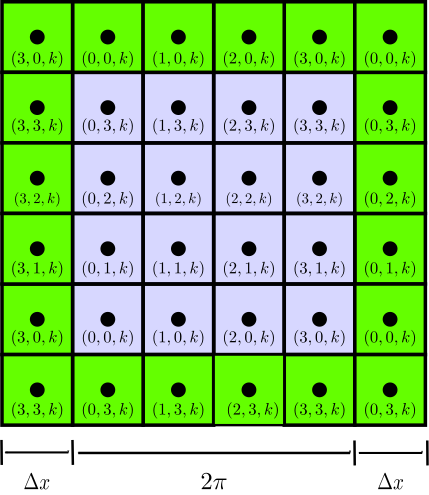
\includegraphics[height=0.35\textheight]{media/rk4/periodic-BCs}
    \caption{Ghost cell examples for $N=4$}
    \label{fig:ghost-cell-example}
\end{figure}

Lastly, after every time step the location of the coordinate point $x$ is
checked to ensure it is still within the domain $0 \leq x_{1}, x_{2}, x_{3}
\leq 2\pi$. Again since the ALES code is periodic, the location of the
coordinate point can be easily adjusted by either adding $2\pi$ for cases
where $x<0$ or subtracting $2\pi$ for cases where $x>0$, namely
\begin{equation}
    x = 
    \begin{cases}
        x           \text{\hspace{1.3cm}if $ 0 \leq x \leq 2\pi$}  \\
        x + 2\pi    \text{\hspace{0.3cm}if $ x < 0$}  \\
        x - 2\pi    \text{\hspace{0.3cm}if $ x > 2\pi$}     \\
    \end{cases}
\end{equation}
An two-dimensional example of how the location of $x$ is adjusted in the
forwards and backwards tracking code can be seen in
Fig~(\ref{fig:location-adjustment}), where we can see how the coordinate
point is relocated to opposite side of the domain.
\begin{figure}[H]
    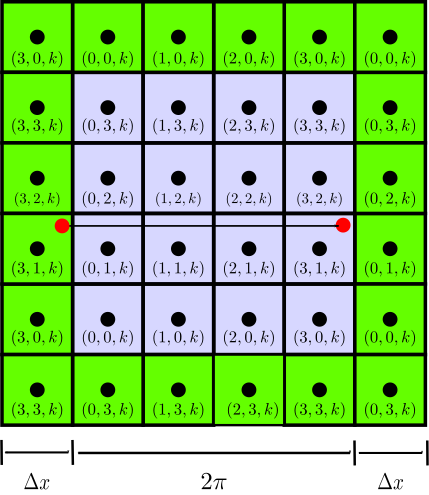
\includegraphics[height=0.35\textheight]{media/rk4/location-adjustment}
    \caption{Example of how the $x$ location is adjusted using periodic B.C.s}
    \label{fig:location-adjustment}
\end{figure}

\subsection{RK4 test} 
Next, we use the numerical schemes described above to
quantify the performance of the backwards tracking tool. First a random
coordinate point $\mathbf{x}=(x_{1}, x_{2}, x_{3})$ initially located on a
grid point is advected forward in time using the forward RK4 scheme and the
velocities from the ALES simulation, storing the solution for the three
coordinate locations after every time step. After the forward in time
reaches the inputted number of time steps, it writes a file with the times
and locations associated with that point. Next, the backwards tracking
subroutines reads in the last entry of the forward file as the initial
condition. Again the backwards tracking subroutine runs for a set number of
time steps storing the times and locations for each step. For testing
purposes the coordinate point was advected for 500 time steps which is
approximately five times as many times required for our analysis. Moreover,
velocity fields from a Basic Smagorinsky (i.e., $C_{DS} =0$) simulation
calculated using three different grids of $N=$32, 64 , and 128 were used in
the testing.  Additionally, not only was the back tracking test performed
using three different grids, each grid was tested five times, giving a
total number of 15 test. Therefore the results presented in
Figs.(\ref{fig:back-tracking-32}-\ref{fig:back-tracking-128}) show the
cases with the largest disparity at $t=0$.  

The following results shown in Fig.~(\ref{fig:back-tracking-32}) show the
results for $N=32$. The plots represent the evolution of a point going
backwards in time, therefore along the x-axis the time steps start at the
final time step ($t=t_{0} + 500 \Delta t$) and advance towards the initial
time $t=t_{0}$.  
\begin{figure}[H]
    \begin{subfigure}[H]{0.45\textwidth}
        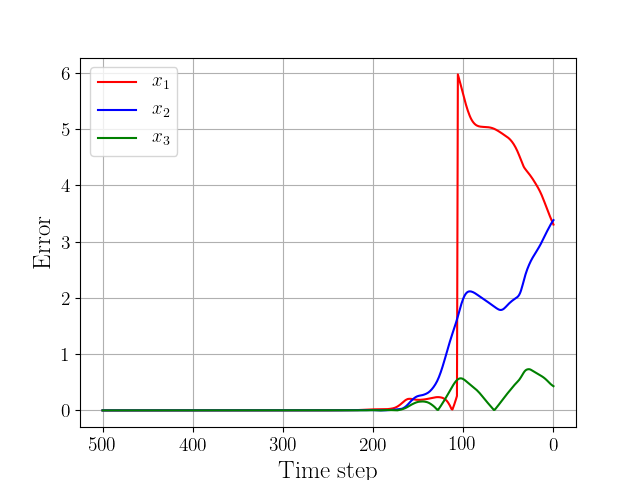
\includegraphics[height=2.5in]{media/rk4/run-32/error-32.png}
        \caption{Error for $N=32$}
    \end{subfigure}
    ~
    \begin{subfigure}[H]{0.45\textwidth}
        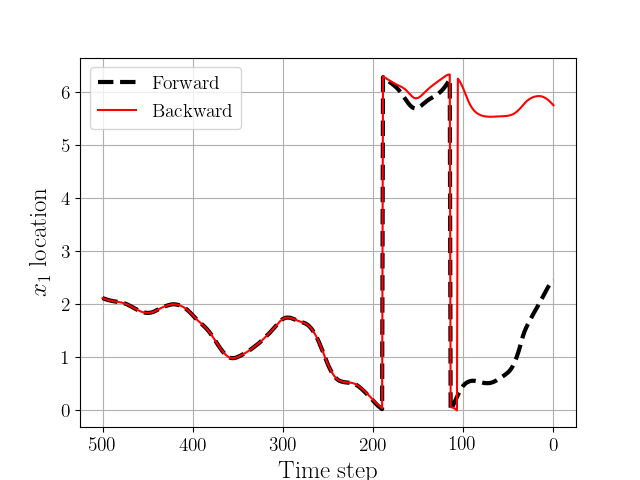
\includegraphics[height=2.5in]{media/rk4/run-32/x1-32-tracking.png}
        \caption{$x_{1}$ location}
    \end{subfigure}
    \newline
    \begin{subfigure}[H]{0.45\textwidth}
        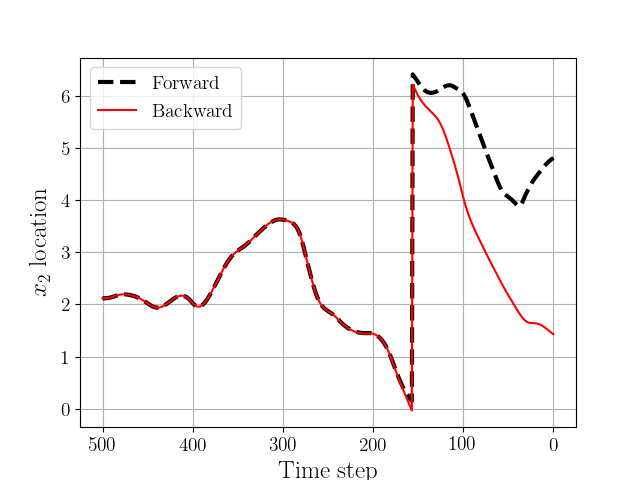
\includegraphics[height=2.5in]{media/rk4/run-32/x2-32-tracking.png}
        \caption{$x_{2}$ location}
    \end{subfigure}
    ~
    \begin{subfigure}[H]{0.45\textwidth}
        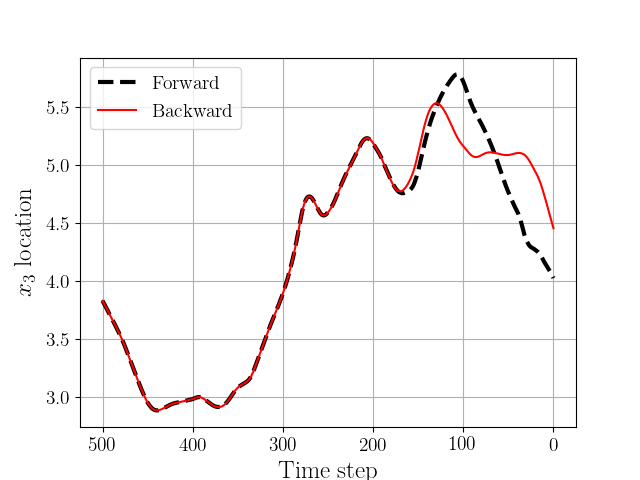
\includegraphics[height=2.5in]{media/rk4/run-32/x3-32-tracking.png}
        \caption{$x_{3}$ location}
    \end{subfigure}
    \caption{Results for $N=32$}
    \label{fig:back-tracking-32}
\end{figure}
Key observations:
\begin{itemize}
    \item The back tracking appears to be very accurate for the first $\sim
        200$ time steps, even at a low spatial and temporal resolution.
        However, at $t=t_{0}$ the tracking is not even close and we are at
        a completely different part of the domain all together.
    \item It appears that once deviation occurs the subroutine almost
        immediately starts following another point since the difference
        just continues to grow. This is not surprising since this is what
        we expected and the reason we are verifying the subroutine.
    \item The error appears to be growing over time as we predicted in the
        phone call, therefore the longer we track the more inaccurate are
        coordinate location becomes. However, given how quickly blowup
        occurs this method is still a valid approach for tracking.

\end{itemize}

The following results shown in Fig.~(\ref{fig:back-tracking-64}) represent
the solution for $N=64$ (\emph{\textbf{note the scale factor on the
y-axis of the error plot}}).
\begin{figure}[H]
    \begin{subfigure}[H]{0.45\textwidth}
        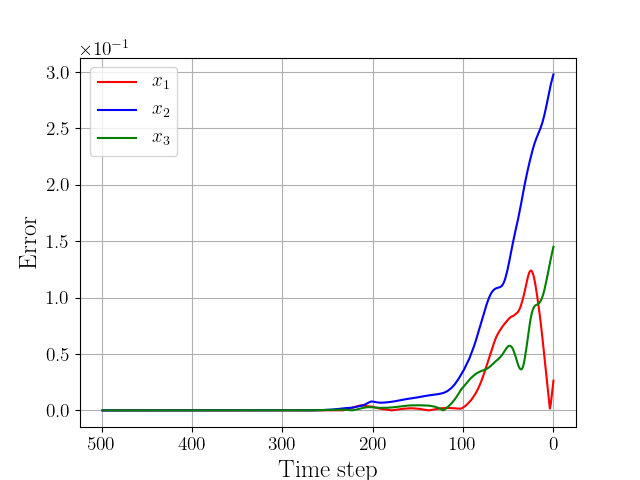
\includegraphics[height=2.5in]{media/rk4/run-64/error-64.png}
        \caption{Error for $N=64$}
    \end{subfigure}
    ~
    \begin{subfigure}[H]{0.45\textwidth}
        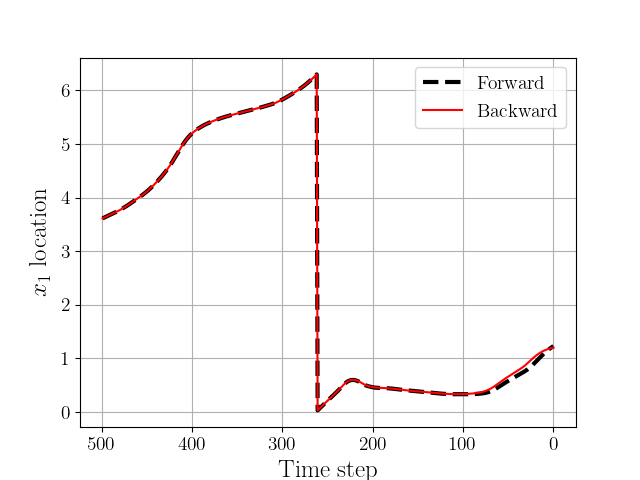
\includegraphics[height=2.5in]{media/rk4/run-64/x1-64-tracking.png}
        \caption{$x_{1}$ location}
    \end{subfigure}
    \newline
    \begin{subfigure}[H]{0.45\textwidth}
        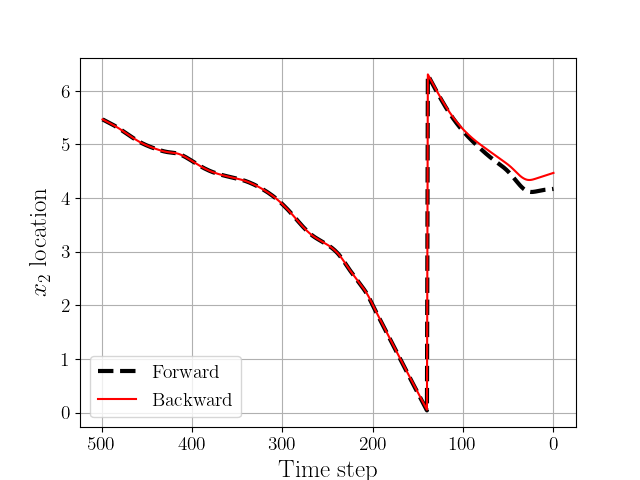
\includegraphics[height=2.5in]{media/rk4/run-64/x2-64-tracking.png}
        \caption{$x_{2}$ location}
    \end{subfigure}
    ~
    \begin{subfigure}[H]{0.45\textwidth}
        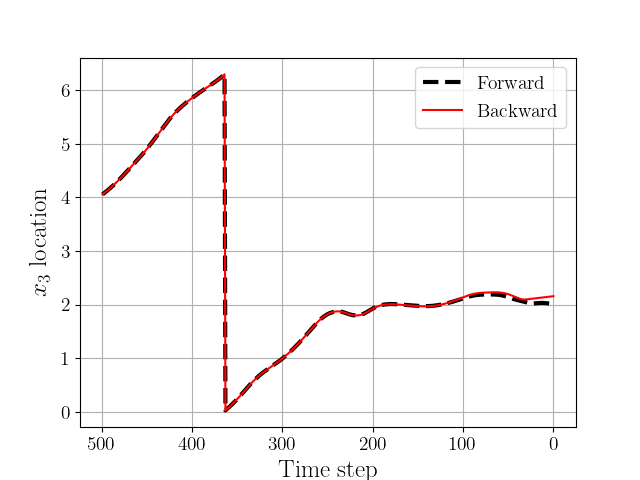
\includegraphics[height=2.5in]{media/rk4/run-64/x3-64-tracking.png}
        \caption{$x_{3}$ location}
    \end{subfigure}
    \caption{Results for $N=64$}
    \label{fig:back-tracking-64}
\end{figure}
Key observations:
\begin{itemize}
    \item Here we can see that an increase in the spatial and temporal
        resolutions greatly increase the subroutines performance. Doubling
        the grid points reduces the error by a factor of $\sim20$ (i.e., $6/0.3$).
    \item With $N=64$ the back tracking appears to be accurate up to $\sim
        400$ time steps.
\end{itemize}

The following results shown in Fig.~(\ref{fig:back-tracking-64}) represent
the solution for $N=128$ (\emph{\textbf{note the scale factor on the
y-axis of the error plot}}).

\begin{figure}[H]
    \begin{subfigure}[H]{0.45\textwidth}
        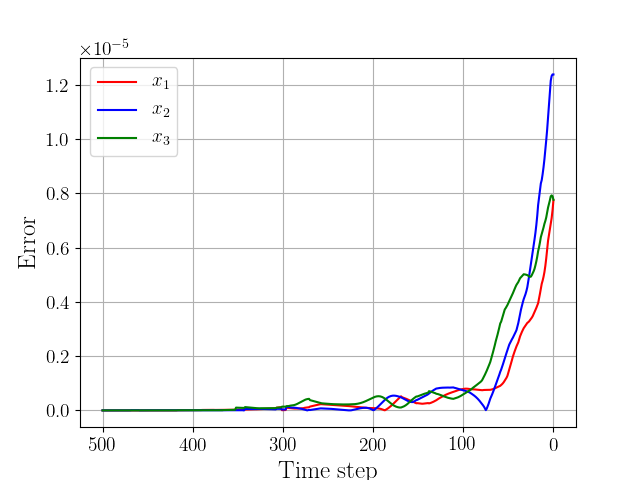
\includegraphics[height=2.5in]{media/rk4/run-128/error-128.png}
        \caption{Error for $N=128$}
    \end{subfigure}
    ~
    \begin{subfigure}[H]{0.45\textwidth}
        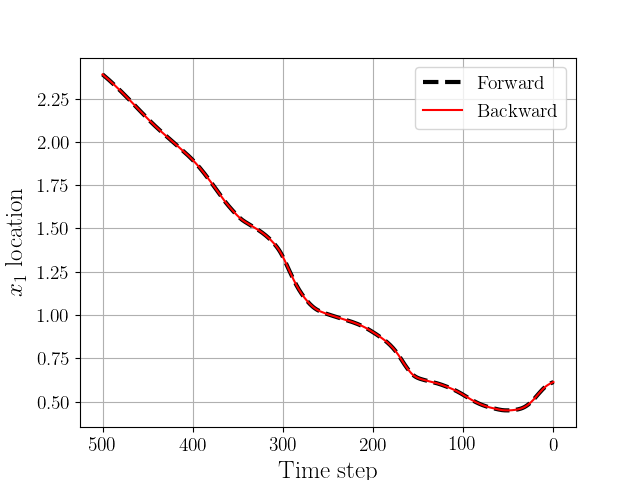
\includegraphics[height=2.5in]{media/rk4/run-128/x1-128-tracking.png}
        \caption{$x_{1}$ location}
    \end{subfigure}
    \newline
    \begin{subfigure}[H]{0.45\textwidth}
        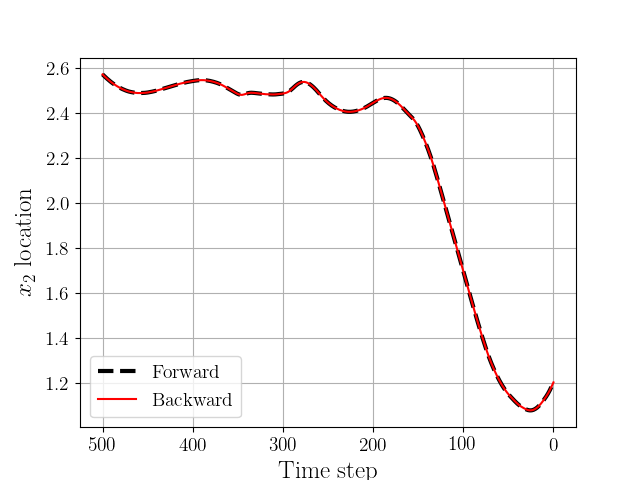
\includegraphics[height=2.5in]{media/rk4/run-128/x2-128-tracking.png}
        \caption{$x_{2}$ location}
    \end{subfigure}
    ~
    \begin{subfigure}[H]{0.45\textwidth}
        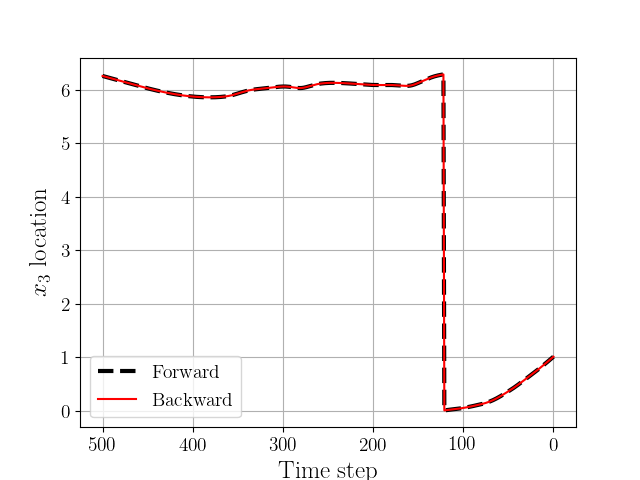
\includegraphics[height=2.5in]{media/rk4/run-128/x3-128-tracking.png}
        \caption{$x_{3}$ location}
    \end{subfigure}
    \caption{Results for $N=128$}
    \label{fig:back-tracking-128}
\end{figure}
Key observations:
\begin{itemize}
    \item Again we can see the error accumulates in time, as we predicted,
            however it is obvious that an increase in resolution leads to
            increase in the number of time steps we can track back in time. 
    \item With $N=128$ we can back track very accurately for $\sim 500$
        time steps.
\end{itemize}
\newpage
Lastly, we can zoom in on the first $200$ time steps $t=t_{0}+500\Delta t
\rightarrow t = t_{0} + 300\Delta t$ of backwards tracking results in order
to gain further knowledge of the accuracy of the back tracking performance.
Starting with the results of $N=32$ shown in
Fig.~(\ref{fig:back-tracking-32-2}) (\emph{\textbf{note the scale factor on the
y-axis of the error plot}}).
\begin{figure}[H]
    \begin{subfigure}[H]{0.45\textwidth}
        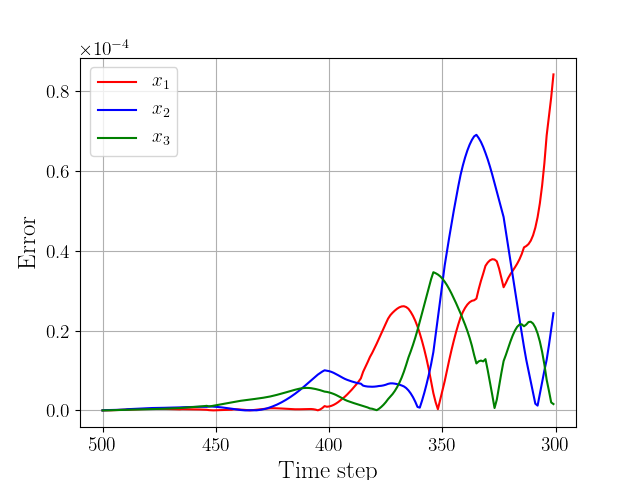
\includegraphics[height=2.5in]{media/rk4/run-32/error-32-2.png}
        \caption{Error for $N=32$}
    \end{subfigure}
    ~
    \begin{subfigure}[H]{0.45\textwidth}
        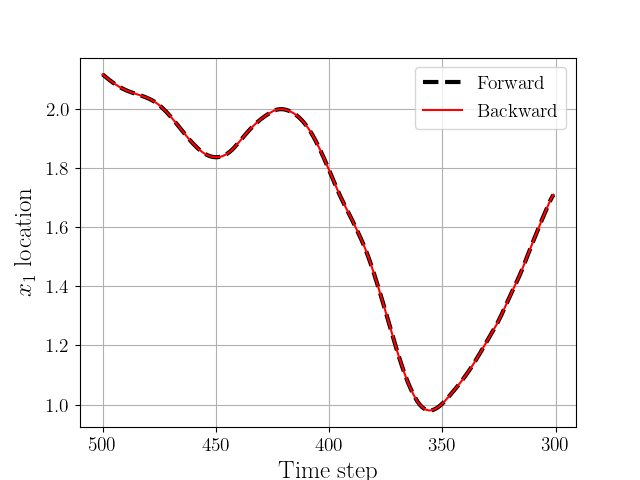
\includegraphics[height=2.5in]{media/rk4/run-32/x1-32-tracking-2.png}
        \caption{$x_{1}$ location}
    \end{subfigure}
    \newline
    \begin{subfigure}[H]{0.45\textwidth}
        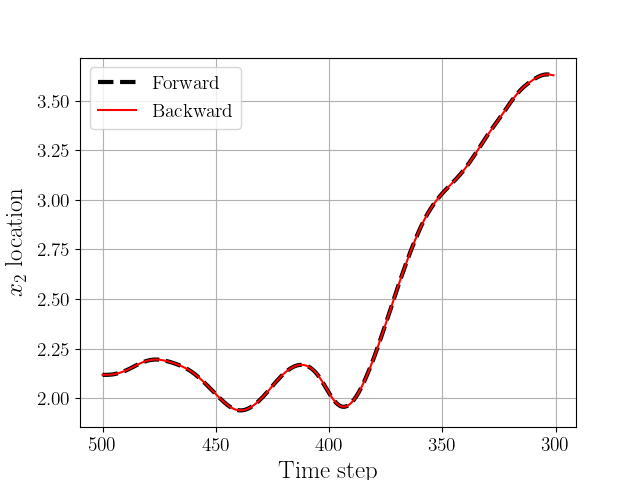
\includegraphics[height=2.5in]{media/rk4/run-32/x2-32-tracking-2.png}
        \caption{$x_{2}$ location}
    \end{subfigure}
    ~
    \begin{subfigure}[H]{0.45\textwidth}
        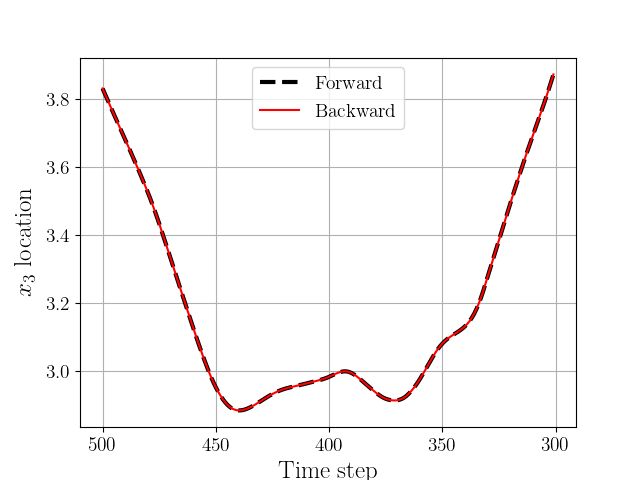
\includegraphics[height=2.5in]{media/rk4/run-32/x3-32-tracking-2.png}
        \caption{$x_{3}$ location}
    \end{subfigure}
    \caption{Results for $N=32$}
    \label{fig:back-tracking-32-2}
\end{figure}
\newpage

Next, we have the results for $N=64$ shown in
Fig.~(\ref{fig:back-tracking-64-2}) (\emph{\textbf{note the scale factor on the
y-axis of the error plot}}).
\begin{figure}[H]
    \begin{subfigure}[H]{0.45\textwidth}
        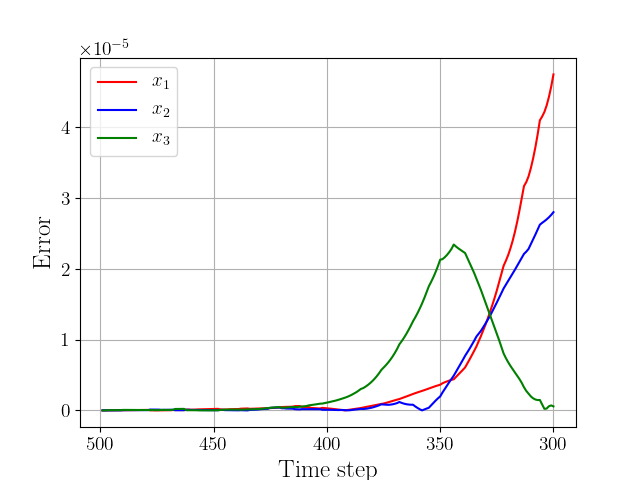
\includegraphics[height=2.5in]{media/rk4/run-64/error-64-2.png}
        \caption{Error for $N=64$}
    \end{subfigure}
    ~
    \begin{subfigure}[H]{0.45\textwidth}
        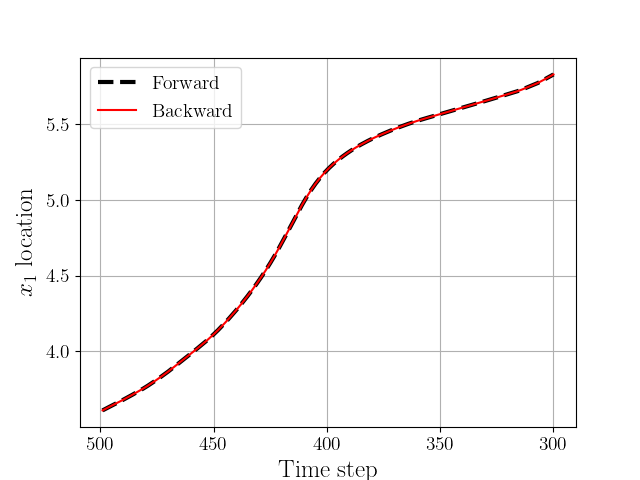
\includegraphics[height=2.5in]{media/rk4/run-64/x1-64-tracking-2.png}
        \caption{$x_{1}$ location}
    \end{subfigure}
    \newline
    \begin{subfigure}[H]{0.45\textwidth}
        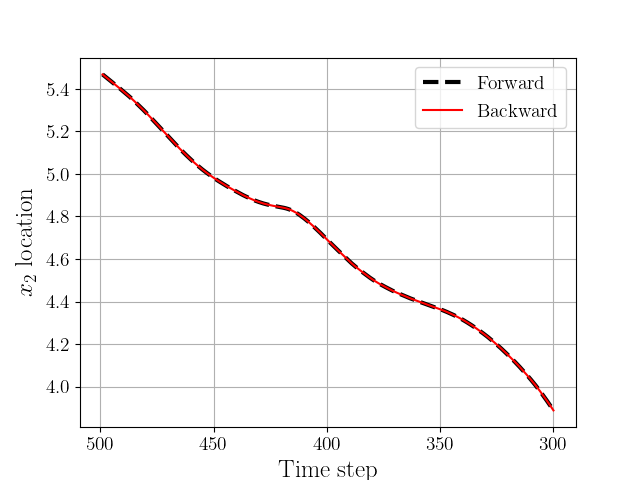
\includegraphics[height=2.5in]{media/rk4/run-64/x2-64-tracking-2.png}
        \caption{$x_{2}$ location}
    \end{subfigure}
    ~
    \begin{subfigure}[H]{0.45\textwidth}
        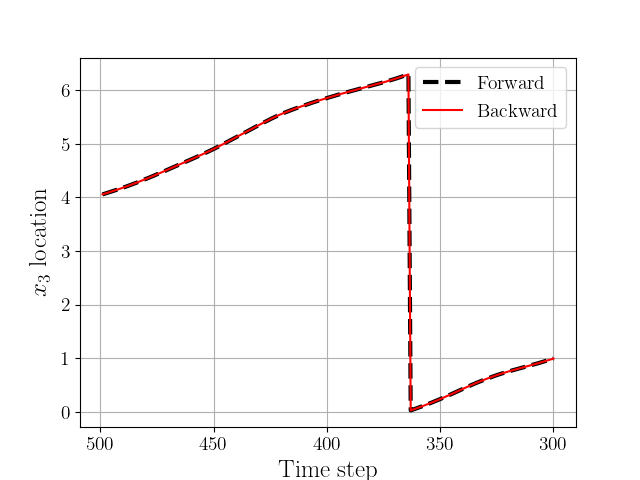
\includegraphics[height=2.5in]{media/rk4/run-64/x3-64-tracking-2.png}
        \caption{$x_{3}$ location}
    \end{subfigure}
    \caption{Results for $N=64$}
    \label{fig:back-tracking-64-2}
\end{figure}
\newpage
Lastly, we have the results for $N=128$ shown in
Fig.~(\ref{fig:back-tracking-128-2}) (\emph{\textbf{note the scale factor on the
y-axis of the error plot}}).
\begin{figure}[H]
    \begin{subfigure}[H]{0.45\textwidth}
        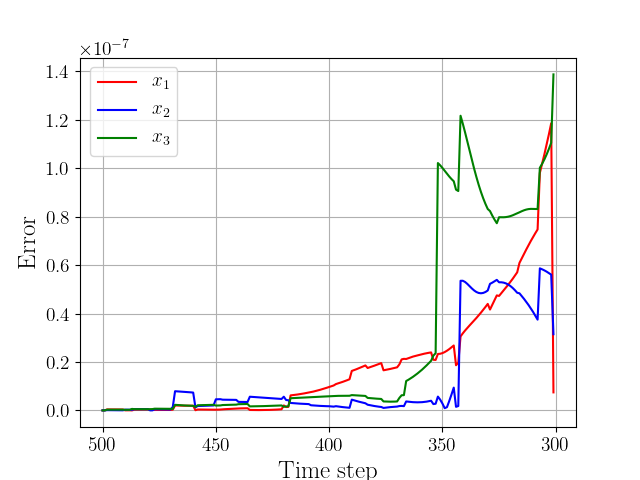
\includegraphics[height=2.5in]{media/rk4/run-128/error-128-2.png}
        \caption{Error for $N=128$}
    \end{subfigure}
    ~
    \begin{subfigure}[H]{0.45\textwidth}
        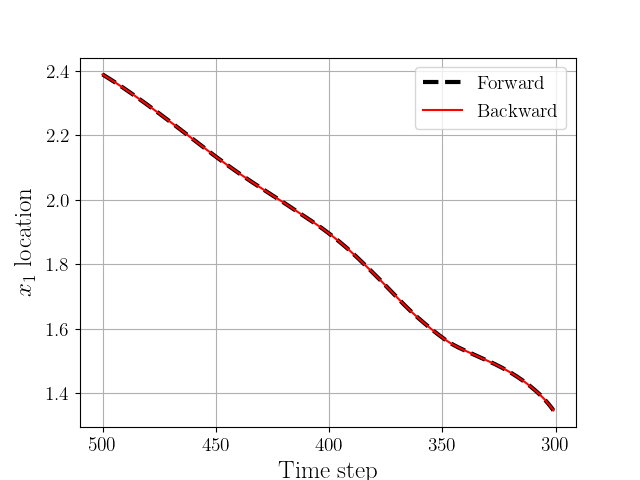
\includegraphics[height=2.5in]{media/rk4/run-128/x1-128-tracking-2.png}
        \caption{$x_{1}$ location}
    \end{subfigure}
    \newline
    \begin{subfigure}[H]{0.45\textwidth}
        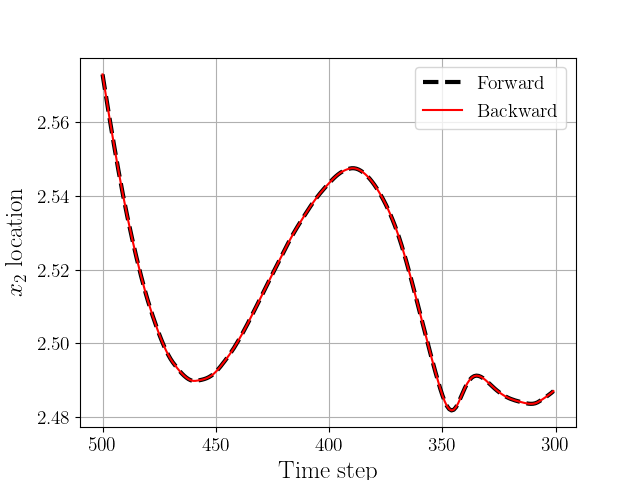
\includegraphics[height=2.5in]{media/rk4/run-128/x2-128-tracking-2.png}
        \caption{$x_{2}$ location}
    \end{subfigure}
    ~
    \begin{subfigure}[H]{0.45\textwidth}
        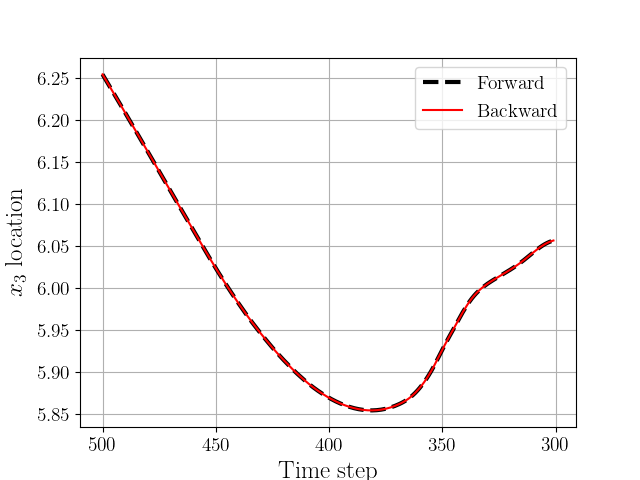
\includegraphics[height=2.5in]{media/rk4/run-128/x3-128-tracking-2.png}
        \caption{$x_{3}$ location}
    \end{subfigure}
    \caption{Results for $N=64$}
    \label{fig:back-tracking-128-2}
\end{figure}
\newpage
The last set of results are used to highlight to accumulation of error over
time, done by plotting error versus time step on a semi-logy scale for the
three cases.
\begin{figure}[H]
    \begin{subfigure}[H]{0.45\textwidth}
        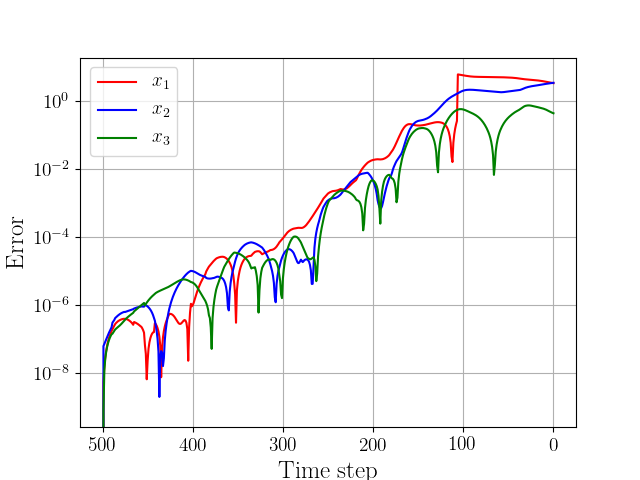
\includegraphics[height=2.5in]{media/rk4/run-32/error-32-log.png}
        \caption{Semi-logy error for $N=32$}
        \label{fig:error-32-semilogy}
    \end{subfigure}
    ~
    \begin{subfigure}[H]{0.45\textwidth}
        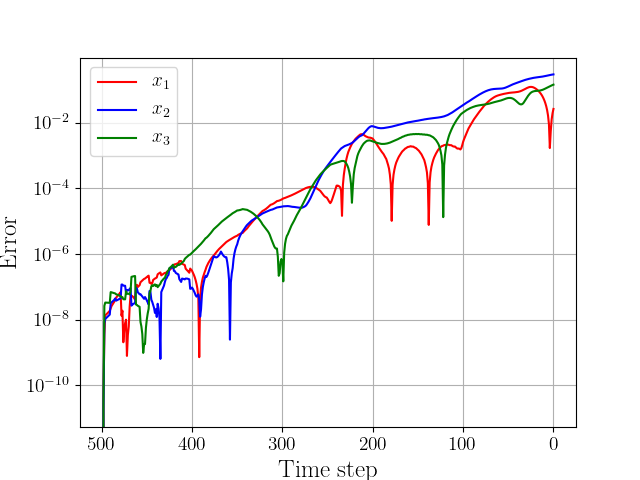
\includegraphics[height=2.5in]{media/rk4/run-64/error-64-log.png}
        \caption{Semi-logy error for $N=64$}
        \label{fig:error-64-semilogy}
    \end{subfigure}
    \begin{subfigure}[H]{0.45\textwidth}
        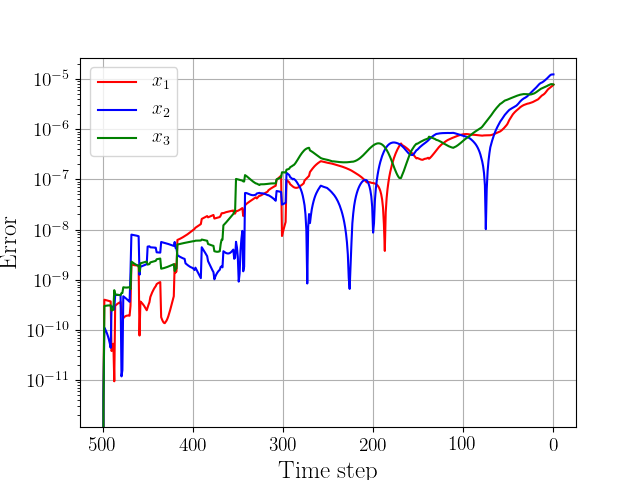
\includegraphics[height=2.5in]{media/rk4/run-128/error-128-log.png}
        \caption{Semi-logy error for $N=128$}
        \label{fig:error-128-semilogy}
    \end{subfigure}
    \caption{Semi-logy error study}
\end{figure}
Key observation:
\begin{itemize}
    \item Clearly the error accumulates over time. 
    \item If we want to take a conservative approach and start using 
            $N=128$ grid points, then even tracking back $\sim100$ time
            steps we can expect an error of $\sim 10^{-8}$, which is
            comparative to what we would expect with a fourth order time
            stepping method with $\Delta t \sim 10^{-2}$ 
            (i.e., $(\Delta t)^{4} \sim 10^{-8}$).
\end{itemize}

